\lecture[0]{Introduction}{lec:intro}

\title{Introduction}
\subtitle{Getting started}

\date{\today}

\begin{frame}
\maketitle
\end{frame}

\section{Forward}
\begin{frame}{Some note about these slides}
\begin{itemize}
    \item These slides were prepared during my sabbatical leave.  I am grateful to Washington University, McKelvey School of Engineering, and the Department of Computer Science and Engineering for sponsoring my sabbatical.
    \item There are some typographical conventions used in these slides, as follows.
    \begin{itemize}
        \item Some text includes hyperlinks to material you can find on the Internet, such as \href{https://en.wikipedia.org/wiki/Hyperlink}{this}.
        \item Where a larger idea or presentation cites material on the Internet, that link will often appear at the end of the material. \LinkArrow{https://en.wikipedia.org/wiki/Wikipedia:Citing_sources}
        \item Where images appear without citation, they are available for \emph{free use} or fall under the \href{https://en.wikipedia.org/wiki/Fair_use}{\emph{fair use}} clause for copyright material. \LinkArrow{https://fas.org/irp/crs/RL31423.pdf}
    \end{itemize}
    \item Errors found in this material are my fault.  Please bring errors to \href{mailto:cytron@wustl.edu}{my attention}, thanks!
\end{itemize}
\end{frame}
\section{Instructor}
\begin{frame}{Your professor}{Brief bio}
\begin{itemize}
    \item Ron Cytron
    \begin{itemize}
        \item You can call me \emph{Ron}
        \item Last name pronounced sit'-run
    \end{itemize}
    \item Undergrad at Rice University
    \item Graduate MS and PhD at University of Illinois
    \item Primary research interests
    \begin{itemize}
        \item Programming languages and compilers
        \item Runtime systems
        \item Computer architecture
    \end{itemize}
    \item So how did I get to Quantum Computing?
\end{itemize}
    
\end{frame}

\section{Background}
\begin{frame}{Curiosity}{And I had a lot of help $\ldots$}
\begin{itemize}
    \item Walter Buhro -- student in CSE 131 but also physics major
    \item Nathan Mester -- we studied this material over a summer
    \item Then I got serious
    \begin{itemize}
        \item Arthur Rattew
        \item Collin Szczepanski
        \item Finn Voichick
    \end{itemize}
\end{itemize}
    
\end{frame}

\begin{frame}{Quantum Computing}{Inherently multidisciplinary}
\begin{tabular}{cc}
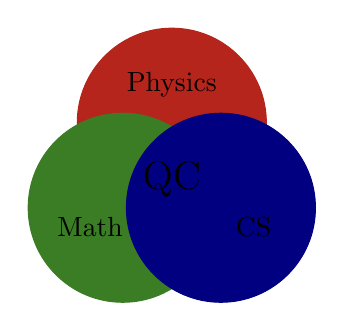
\begin{tikzpicture}[scale=0.6]
%  \begin{scope}
    \fill<1>[color=BrickRed]   ( 90:1.2) circle (2);
    \draw[color=BrickRed]   ( 90:1.2) circle (2);
    \fill<2>[color=OliveGreen] (210:1.2) circle (2);
    \draw[color=OliveGreen] (210:1.2) circle (2);
    \fill<3>[color=NavyBlue]  (330:1.2) circle (2);
    \draw[color=NavyBlue]  (330:1.2) circle (2);
%  \end{scope}
  \node<1-> at ( 90:2)    {Physics};
  \node<2-> at ( 210:2)   {Math};
  \node<3-> at ( 330:2)  {CS};
  \node<4-> [font=\Large] {QC};
\end{tikzpicture}
&
\begin{minipage}[b]{0.5\textwidth}
\begin{itemize}
    \item<1->{\textcolor<1>{BrickRed}{Physics is the study of the observable universe}}
    \item<2->{\textcolor<2>{OliveGreen}{Math is the study of logic and reasoning}}
    \item<3->{\textcolor<3>{NavyBlue}{Computer science solves problems using computation}}
\end{itemize}

\end{minipage}
\end{tabular}
\BigSkip{}
\only<4>{
\BigSkip{}
Quantum Computing combines all of these disciplines}
\only<1>{\ColorR{We study physics so as to understand and believe in quantum behavior}}
\only<2>{\ColorG{Quantum values and gates can be represented using linear algebra}}
\only<3>{\ColorB{Computer science lets us reason about the problems we can solve}}
\end{frame}

\begin{frame}{Prerequisites}
\begin{description}
    \item[Linear and Matrix Algebra] We use this heavily.  You must be familiar with row and column vectors, matrix multiplication, linear systems of equations.
    
    Example:  Math 309
    \item[Probability] Quantum computations are inherently probabilistic.  You need to have some background in probability, but it doesn't have to be extensive.
    
    Examples:  ESE 326 or Math 3200
    \item[Circuits]  We will specify quantum computations using circuit diagrams.  Some familiarity with Boolean algebra and circuit elements depicting Boolean operations is needed.
    
    Examples:  CSE 132 or CSE 260M
\end{description}
\end{frame}
\begin{frame}{Goals}
\begin{itemize}
    \item Understand and be able to construct quantum circuits to solve a problem.
    \item Sufficient background to take quantum information courses in ESE.
    \item Sufficient background to take foundational courses in Math.
\end{itemize}
\end{frame}


\section{Computation}

\def\rcolpic#1{%
\begin{tikzpicture}[overlay]
      \node (steam) at (0.5,-2.5) {
        \includegraphics[width=1.3\textwidth]{0/#1}};
    \end{tikzpicture}
}
\begin{frame}{Computer scientists are (like) cuckoos}{We steal ideas from other disciplines to compute things}

\begin{columns}
\begin{column}{0.7\textwidth}
 We can realize computations using
\begin{itemize}
    \item<1->Steam
    \item<2-> Semiconductor physics
    \item<3-> Gears, sprockets, and springs
    \item<4-> Water
    \item<5-> DNA
    \item<5-> Gravity
    \item<5-> Quantum effects
\end{itemize}
\end{column}
\begin{column}{0.3\textwidth}
    \only<1>{%
        \rcolpic{steam.jpeg}
    }
    \only<2>{%
        \rcolpic{transistor.jpeg}
    }
    \only<3>{%
        \rcolpic{digicomp.jpeg}
    }
    \only<4>{%
        \rcolpic{water.jpeg}
    }
\end{column}
\end{columns}

    
\end{frame}

\begin{frame}{Using gravity to compute square roots}{We steal ideas from other disciplines to compute things}
\only<-4>{\begin{tikzpicture}[overlay]
  \node (myfirstpic) at (9.5,-3) {
  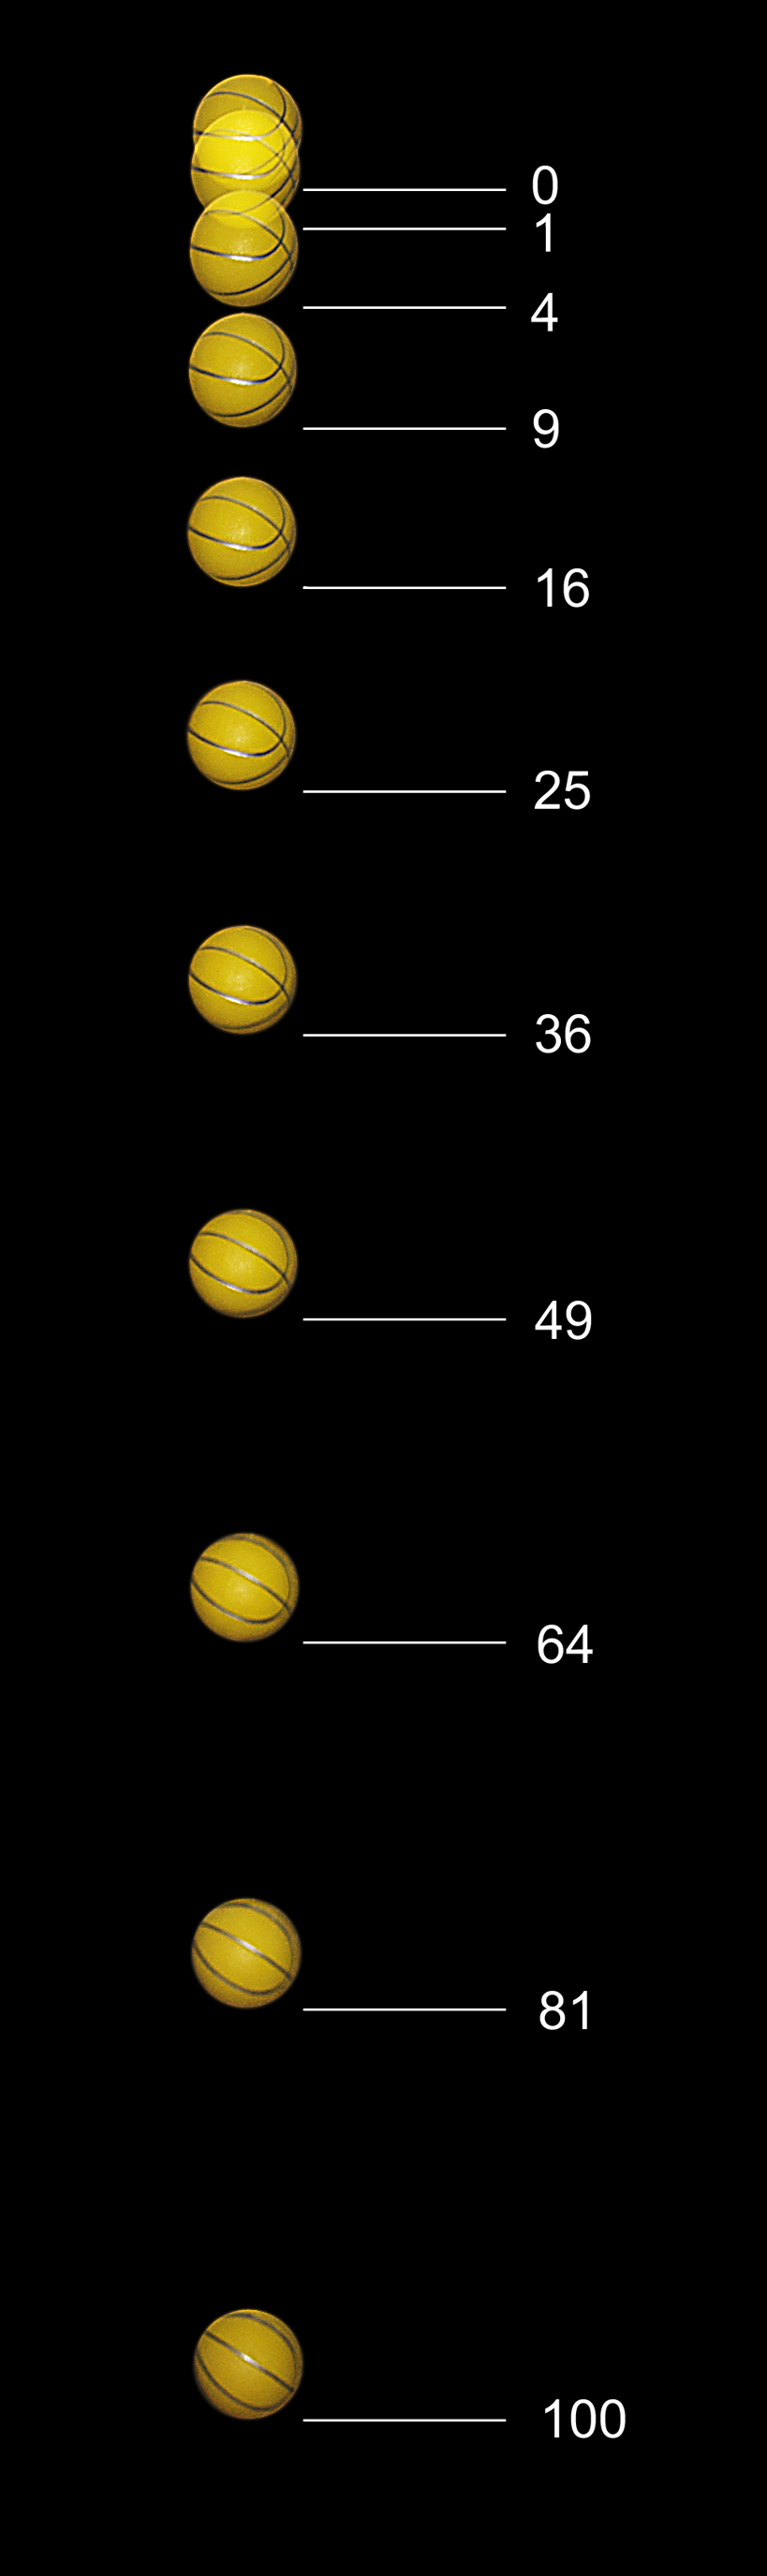
\includegraphics[width=0.15\textwidth]{0/fallingball.jpeg}
  };

\end{tikzpicture}}
\only<1->{How can we use gravity to compute square roots?}

\only<2-3>{We know from physics}
\only<3->{
\begin{eqnarray*}
\only<3>{\ColorR{d} & = & \frac{1}{2} a \ColorG{t}^{2} \\}
\only<4->{\ColorG{t} & = & \sqrt{\frac{2\ColorR{d}}{a}}}
\end{eqnarray*}}
\only<5->{To compute $\sqrt{n}$, we just need to drop a ball from height $\ColorR{d}=\frac{an}{2}$ and measure the time for the ball to hit the ground.}
\only<6->{
\MedSkip{}
Example:
\begin{eqnarray*}
a & = & 9.8 \mbox{ m/$s^2$} \\
n & = & 81 \\
\ColorR{d} & = & an / 2 = 369.9 \mbox{ meters}
\end{eqnarray*}
Takes 9 seconds to drop}
\end{frame}

\begin{frame}{Using DNA to solve Traveling Salesperson\LinkArrow{https://www.jyi.org/2005-september/2005/9/7/fear-not-traveling-salesmen-dna-computing-is-here-to-save-the-day}}{Uses biophysical properties of ligation and electrophoresis}
    
\begin{columns}
    \begin{column}{0.5\textwidth}
        \begin{itemize}
            \item<1-> Each city is represented by a strand of DNA, with a unique first and last part.
            \item<2-> The strand of one city can ligate to the strand of an adjacent city, thus extending the path
            \item<3-> These strands of DNA can be sorted by length using \href{https://en.wikipedia.org/wiki/Gel_electrophoresis}{electrophoresis}, with the shortest acceptable strand encoding the solution.
        \end{itemize}
 
    \end{column}
    \begin{column}{0.5\textwidth}  %%<--- here
     \begin{center}
        \vskip -2.5em
        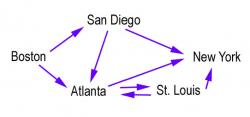
\includegraphics[width=0.9\textwidth]{0/map.jpeg}
     \end{center}
     \only<1->{
        \begin{tabular}{lcl}
            San Diego & = & \texttt{TTG AAA} \\
            Atlanta   & = & \texttt{TTT CTC}
        \end{tabular}
     }
     \only<2->{
        \MedSkip{}
        Possible ligation:
        
        \begin{tabular}{lll}
            \texttt{TTG} & \texttt{AAA} \\
               &  \texttt{TTT} & \texttt{CTC}
        \end{tabular}
     }
     
     \only<3->{
        Diagram of electrophoresis
     }
    \end{column}
\end{columns}

\end{frame}

\begin{frame}{Quantum effect}{Warning:  This material may be mind blowing}
\begin{itemize}
    \item Small particles such as electrons and photons live a very strange existence.
    \item We lack experience or even adequate language language to understand or express how they behave.
    \item However, \href{https://en.wikipedia.org/wiki/Quantum_mechanics}{quantum mechanics} has been extraordinarily successful in predicting the outcomes of quantum events.
    \item Einstein did not (want to) believe that his own theories were complete concerning their behavior.\LinkArrow{https://en.wikipedia.org/wiki/Bohr-Einstein_debates}
\end{itemize}
\only<2->{
\begin{description}
    \item[Einstein:]  God does not play dice with the universe.
    \item[Bohr:] Don't tell God what to do with God's dice!
\end{description}}

\only<3->{\alert{
We can use quantum effect to compute interesting results.   In this course we look at various problems and develop solutions based on quantum effects.}}

\end{frame}

\section{Logistics}

\begin{frame}{Course overview and logistics}{You are responsible for this knowledge}
\begin{itemize}
    \item Lecture
    \item Homework
    \item Exams
    \item Group work
    \item Academic integrity
    \item How to get help
\end{itemize}
\end{frame}
